% Define the document type
\documentclass[landscape]{slides}

% Import latin characters
\usepackage[latin1]{inputenc}

% Import package for graphics inclusion
\usepackage{graphicx}

% Use Colors
\usepackage{color}

% URLify stuff
\usepackage{hyperref}

% Define author
\author{Marcos Daniel Marado Torres\\ANSOL.org}

% Define title
\title{Censura e Privacidade na Web}

% Define date
\date{O Crime no s�c. XXI}

% begin document
\begin{document}

% TITLE
% p1

\begin{slide}
	\Huge{\maketitle}
\end{slide}


%%% Ordenado

% > > 1 - H� privacidade na web?
% p2
\begin{slide}
	\begin{center}
		\begin{LARGE}
			\begin{itemize}
				\item{} \textcolor{red}{H� privacidade na web?}
				\item{} Privacidade, Seguran�a, Censura
				\item{} Ter privacidade
			\end{itemize}
		\end{LARGE}
	\end{center}
\end{slide}

% > > 1.1 web vs. Internet vs computing
\begin{slide}
	\begin{LARGE}
		H� privacidade na web?
		\begin{center}
			Web \\ vs. \\ Internet \\ vs. \\ Computing
		\end{center}
	 \end{LARGE}
\end{slide}

% no time in 30mins...

% \begin{slide}
% 	H� privacidade na web?
% 	\begin{itemize}
% 		\item{} technology should be an enabler: \\ use what you want, how you want
% 		\item{} who you are vs. what you do
% 	\end{itemize}
% \end{slide}

\begin{slide}
	H� privacidade na web?
	\begin{itemize}
		\item{} No privacy - the Facebook example
		\item{} Hybrid privacy - the Amazon example
		\item{} Privacy - Local storage, local services
		\item{} Local privacy needs local security
	\end{itemize}
\end{slide}

\begin{slide}
		H� privacidade na web?
\begin{itemize}
\item{} Aquilo que hoje � privado amanh� pode ser p�blico
\item{} Aquilo que hoje � p�blico nunca mais ser� privado
\item[$\diamond$]{} Os dados t�m dono, mas o dono n�o manda na forma como eles s�o usados
\item[$\diamond$]{} Girls Around Me
\end{itemize}
\end{slide}
% (Girls Around Me)
% http://news.cnet.com/8301-31322_3-57408165-256/girls-around-me-and-the-end-of-internet-innocence/?part=rss&subj=news&tag=title

% > > 2 - Privacidade vs. Seguran�a
% p6
\begin{slide}
	\begin{center}
		\begin{LARGE}
			\begin{itemize}
				\item{} H� privacidade na web?
				\item{} \textcolor{red}{Privacidade, Seguran�a, Censura}
				\item{} Ter privacidade
			\end{itemize}
		\end{LARGE}
	\end{center}
\end{slide}

% > > 2.1 richelieu
\begin{slide}
	Privacidade, Seguran�a, Censura
	\begin{quotation}
		Give me six lines written by the most honorable of men, and I will find an excuse in them to hang him. 
	\end{quotation}
	\hfill --- Cardinal Richelieu 
\end{slide}

% http://diariodigital.sapo.pt/news.asp?id_news=445845
\begin{slide}
	\center{
\includegraphics{videovigilancia.png}}
\end{slide}

% > > 2.2 copyright infringement no YouTube
\begin{slide}
	\begin{quotation}
		sites that contain ``infringing'' material also contain an astounding amount of noninfringing material placed there by artists as part of their legitimate distribution schemes. Take a site like YouTube, with something like a billion files (and about 5 percent of them infringe copyright), which assembles and makes public a body of creative work that is larger than ever dreamt of before. Shut it down? It's as if we've discovered a town that houses the largest library ever built, surrounded by a shantytown of pirated DVDs, and so we propose to bulldoze the whole city. 
	\end{quotation}
	\hfill --- Cory Doctorow

	\hfill \url{http://craphound.com/gbbt/}
\end{slide}

% > > 2.3 Tahir

\begin{slide}
	\center{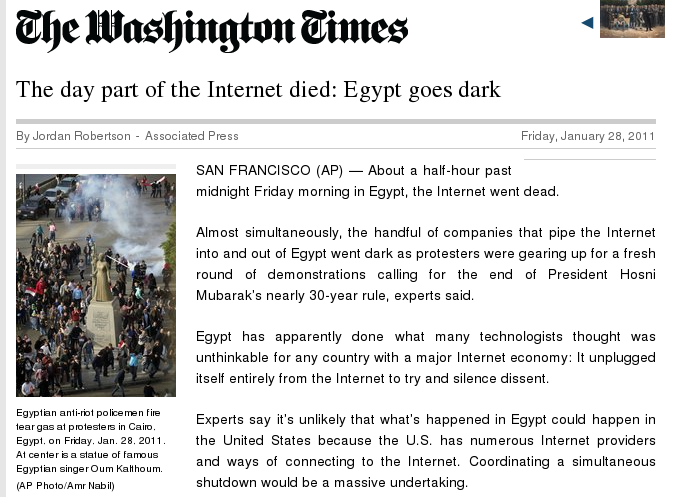
\includegraphics{egypt.png}}
\end{slide}

% > > 2.4 information doesn't want to be free, people do 

\begin{slide}
Privacidade, Seguran�a, Censura
\begin{itemize}
\item{} Information Doesn't Want to be Free, People Do
	\begin{quotation}
		What I am describing is not information freedom. Is it the freedom of individuals to control how information about themselves and their socio-political activities are shared and with whom. And this - like the ability to peacefully assemble and organize - is a prerequisite to the achievement of other important rights. 
	\end{quotation}
	\hfill --- Charli Carpenter
	
	\hfill \tiny{\url{http://duckofminerva.blogspot.pt/2011/01/information-doesnt-want-to-be-free.html}}
\end{itemize}
\end{slide}

% http://yro.slashdot.org/story/12/04/18/1456236/british-mps-propose-censoring-internet-by-default
\begin{slide}
	\center{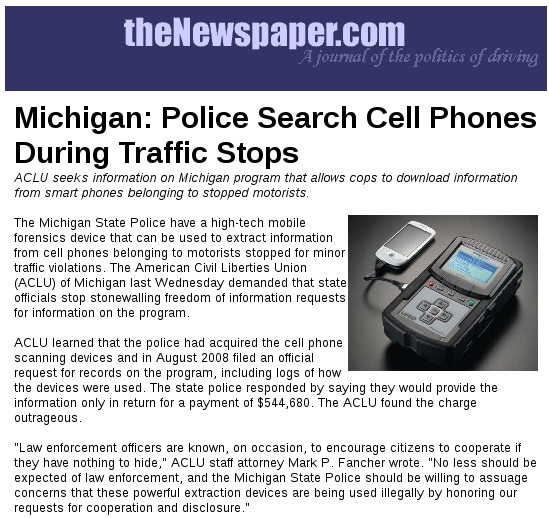
\includegraphics{phones.png}}
\end{slide}


% * CENSURA
% > > * Erasing history - Apagar twitter accounts de protesters do occupywallstreet 

\begin{slide}
	\center{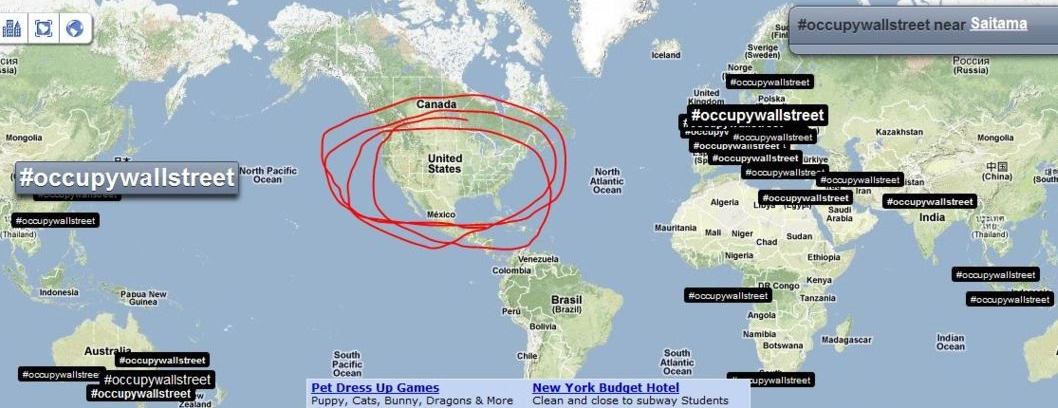
\includegraphics{occupy.jpg}}
\end{slide}

% > > * http://t.co/6x2Swovp
\begin{slide}
	\center{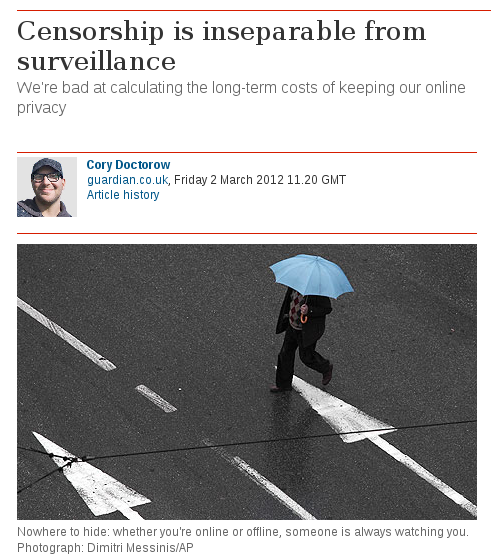
\includegraphics{censorship-surveillance.png}}
\end{slide}

\begin{slide}
	\center{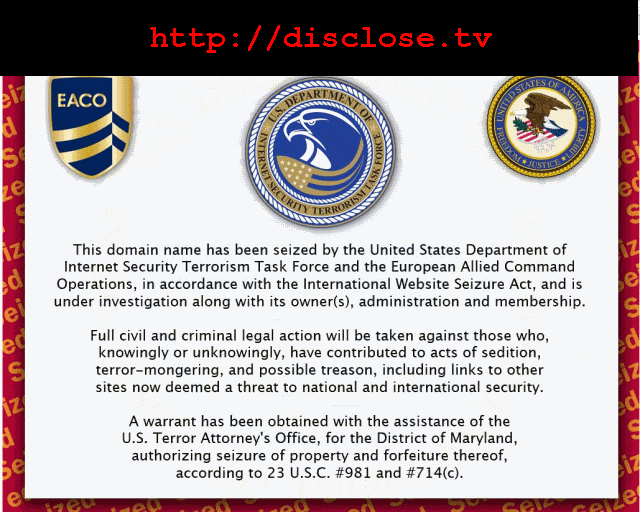
\includegraphics{disclose.png}}
\end{slide}

\begin{slide}
	\center{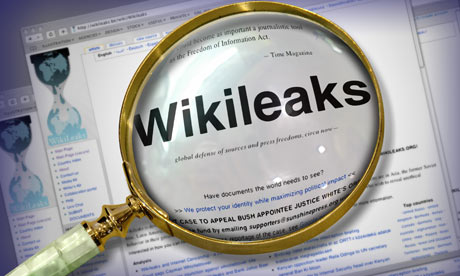
\includegraphics{wikileaks.jpg}}
\end{slide}
	

\begin{slide}
	How to censor an internet connection?
	\begin{itemize}
		\item{} chat vs. blogs, GroovyNotes
		\item{} Gmail/Yahoo Mail
		\item{} \url{http://youtubeproxy.org} (supports YouTube and MySpace)
		\item{} \url{http://thefacebookproxy.com}, \url{http://FacebookProxy360.com}, ...
		\item{} \url{http://www.pendrivelinux.com}
	\end{itemize}
\end{slide}
\begin{slide}
	How to censor an internet connection?
	\begin{itemize}
		\item{} Browse by Proxy
		\item{} Host a Proxy
		\item{} Remote Desktop, VNC, ...
		\item{} DNS queries vs. direct to IP
		\item{} VPN connections
	\end{itemize}
\end{slide}

% * http://tek.sapo.pt/noticias/computadores/receitas_eletronicas_podem_nao_garantir_segur_1235862.html#
\begin{slide}
	\center{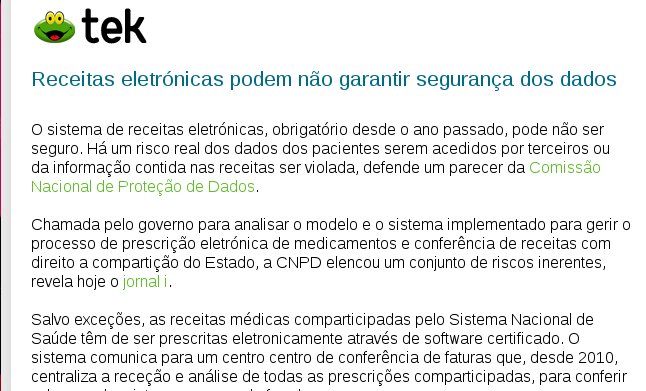
\includegraphics{receitas.png}}
\end{slide}

% No time...
% 
% % > > 2.5 Bursts
% \begin{slide}
% 	\center{
\includegraphics{bursts.jpg}}
% \end{slide}

% > > http://www.publico.pt/Tecnologia/proposta-de-nova-directiva-e-centro-de-combate-reforcam-luta-contra-cibercrime-na-europa-1539966
\begin{slide}
	\center{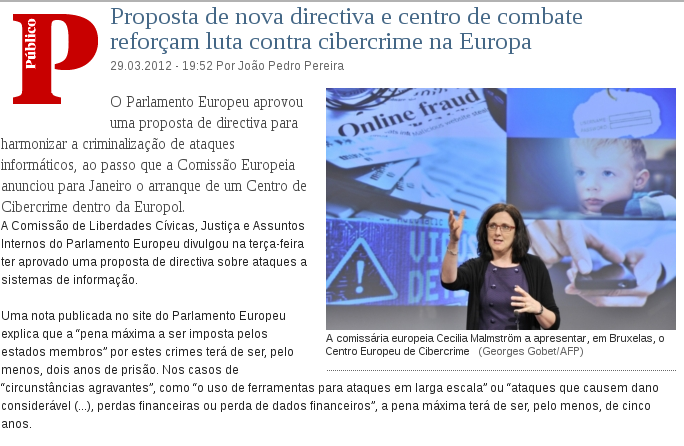
\includegraphics{cibercrime-eu.png}}
\end{slide}

% > http://www.guardian.co.uk/world/2012/apr/01/government-email-social-network-surveillance?intcmp=239
\begin{slide}
	\center{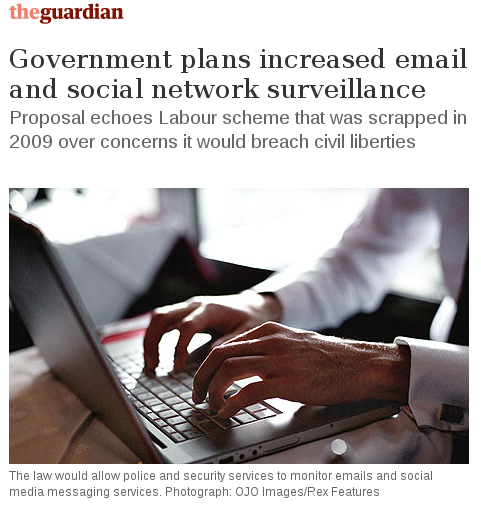
\includegraphics{uk-surveillance.png}}
\end{slide}


% > > 3 - Ter privacidade
% p4
\begin{slide}
	\begin{center}
		\begin{LARGE}
			\begin{itemize}
				\item{} H� privacidade na web?
				\item{} Privacidade, Seguran�a, Censura
				\item{} \textcolor{red}{Ter privacidade}
			\end{itemize}
		\end{LARGE}
	\end{center}
\end{slide}

% > > 3.1 SW Livre
\begin{slide}
	\center{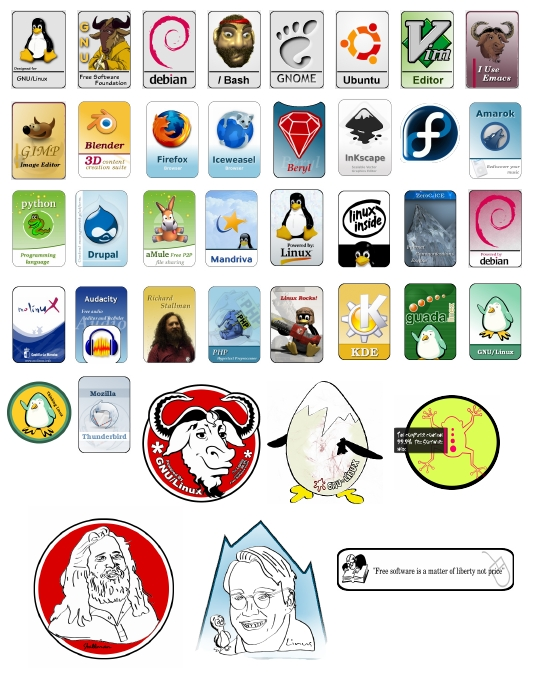
\includegraphics{free.jpg}}
\end{slide}

\begin{slide}
Software Livre � o Software que respeita quatro liberdades:
\begin{itemize}
	\item[\emph{1�}] A liberdade de executar o software, para qualquer uso.
	\item[\emph{2�}] A liberdade de estudar o funcionamento de um programa e de adapt�-lo �s suas necessidades.
	\item[\emph{3�}] A liberdade de redistribuir c�pias.
	\item[\emph{4�}] A liberdade de melhorar o programa e de tornar as modifica��es p�blicas de modo que a comunidade inteira beneficie da melhoria.
\end{itemize}
\end{slide}

% > > 3.6 SAS FSF

\begin{slide}
	\begin{quotation}
		services $[...]$ should not depend on, suggest or encourage use of services which are SaaS; SaaS needs to be replaced by free software.
	\end{quotation}
	\hfill --- Richard Stallman

	\small{\url{http://www.gnu.org/philosophy/network-services-arent-free-or-nonfree.html}}
\end{slide}

\begin{slide}
	\begin{itemize}
		\item{} Termos de Servi�o
		\item{} Pol�ticas de Privacidade
		\item{} Contratos em branco
		\item{} Web de confian�a (pessoas vs. Empresas)
		\item{} Forms desnecess�rios, bugmenot!
		\item{} search history
	\end{itemize}
\end{slide}
\begin{slide}
	\begin{itemize}
		\item{} Logout! (MySpace)
		\item{} Use formatos abertos (ex. hist�rico de edi��es OOXML)
		\item{} Cifre! Mails, disco, backups
		\item{} TOR
		\item{} GNUnet
		\item{} Help us help you: ANSOL, EFF, FFII, ...
	\end{itemize}
\end{slide}

% > > http://www.slideshare.net/gnat/web-meets-world-privacy-and-the-future-of-the-cloud-presentation?type=powerpoint
\begin{slide}
	\begin{quotation}
In 2006 AOL released 20M web queries from 650k users, sampled over three months, to help researchers improve the state of search technology. AOL claimed that the data had been anonymized by turning usernames into unique IDs. However many searches contained identifying information such as addresses, names, and even e-mail messages. The New York Times was able to identify, for example, user 441749 as Thelma Arnold of Lilburn Georgia, who has an interest in numb fingers, 60-ish single man, and dogs that urinate on everything.$[...]$

On the subject of AOL, remember that they tried to anonymize. The privacy loss, while you and I might think was predictable, wasn't deliberate. Shit, as they say, happened.
	\end{quotation}
	\hfill --- Nat Torkington
\end{slide}


% s25
%
\begin{slide}
Desafios:
\begin{itemize}
	\item{} University forces students to use non-private services, social networks, software...
	\item{} Extradi��o UK para USA copyright dom�nio .com
	\item{} Enforcing the law vs. update the law
	\begin{itemize}
		\item{} Piracy vs. Creative Commons \\ (``CC0 is a way of facing 0\% Piracy!'')
		\item{} Lei da C�pia Privada
	\end{itemize}
\end{itemize}
\end{slide}


% http://goo.gl/iMkvY
\begin{slide}
	\center{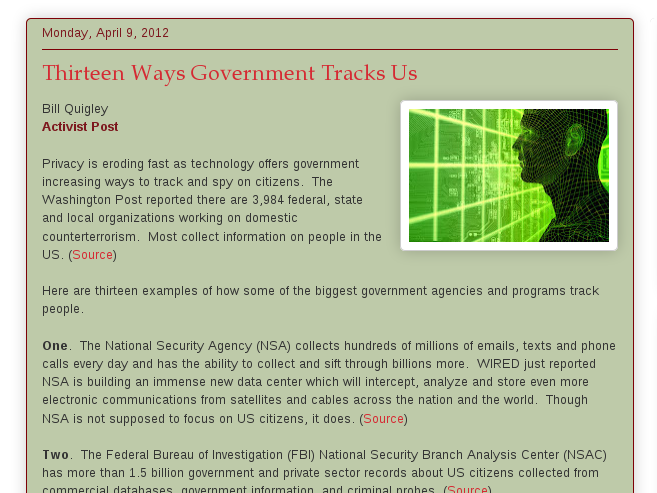
\includegraphics{government.png}}
\end{slide}


% \item{} http://tinyurl.com/6v42r7t - hacktivismo = al caeda do ciber espa�o
\begin{slide}
	\center{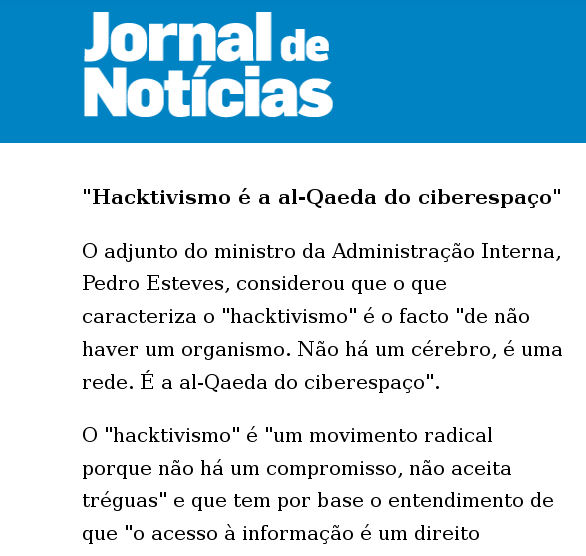
\includegraphics{hactivismo.png}}
\end{slide}


% Information the next Trade War? Data Privacy v CISPA
% http://t.co/gom6Jn3A 
\begin{slide}
	\center{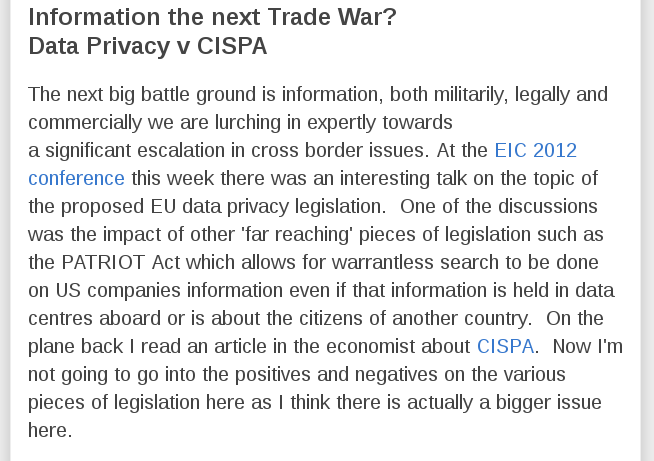
\includegraphics{CISPA.png}}
\end{slide}


% http://yro.slashdot.org/story/12/04/18/1456236/british-mps-propose-censoring-internet-by-default
\begin{slide}
	\center{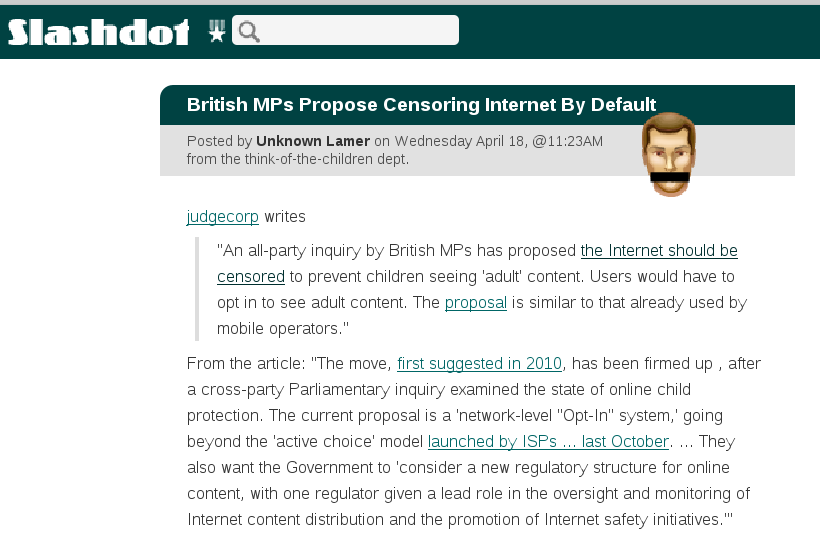
\includegraphics{uk-censorship.png}}
\end{slide}


% > > * http://tinyurl.com/cnpzjav
\begin{slide}
	Futuro:
	\begin{itemize}
		\item{} Do Not Track \& W3C
		\item{} HTTPS Everywhere
		\item{} Regulate Data Brokers
	\end{itemize}
\end{slide}


% :::::::::::

% Stuff to use in a >30mins version of this presentation:
% 
% > > http://m.vanityfair.com/culture/2012/05/internet-regulation-war-sopa-pipa-defcon-hacking
% MORE FROM http://www.slideshare.net/gnat/web-meets-world-privacy-and-the-future-of-the-cloud-presentation?type=powerpoint
% http://arstechnica.com/tech-policy/news/2012/04/patent-trolls-mind-your-own-extra-judicial-business-court-says.ars?clicked=related_right
% http://m.guardian.co.uk/world/2012/apr/07/surveillance-technology-repressive-regimes?cat=world&type=article
% http://spiderplantland.co.uk/sir-olly-c-and-the-case-for-free-speech-in-bexley/
% http://www.zdnet.com/blog/facebook/google-facebook-and-apple-threaten-internet-freedom/11805
% http://expresso.sapo.pt/utilizadores-deviam-exigir-ao-google-e-ao-facebook-os-seus-dados=f719904

% QUEST�ES
\begin{slide}
\center{\Huge{QUEST�ES?}}

\url{http://ANSOL.org} \\
\emph{marcos.marado@ansol.org}
\end{slide}

\end{document}
